% L22.tex
%
% Predrag created file				jul  9 2006
% $Author$ $Date$


\section{Small $L=22$ system {\rpo s}}

\KS\ system $L = 22$ periodic on the full space is small but empirically 
large enough to exhibit persistent chaos.  $L=22$ is a sensible choice 
because In units of mean wavelength the size of this small system is about 
$ \tilde{L}/\sqrt{2}= 2.4758$ 2.5 wavelengths, so the dynamics is 
competition between wavenumbers 2 and 3. Because of the strong $k^4$ 
contraction in \KS\ we expect a small eigenvalues to be significant, rest 
are in the numerical noise. See figure~6 in \refref{Christiansen:97}.

% Davidchack and Crofts 
 We investigate this system in 16 to 64 complex Fourier modes (32 to 
128-dimensional system of real ODEs) truncation, and recheck the results 
by redoing the calculation with the double number of Fourier modes. % 
observe how many digits change. The \eqv\ points are accurate to at least 
to $10^{-11}$. Since Lapack is also double precision accurate, the 
accuracy of the first few eigenvalues is similar, and certainly in excess 
of 6 significant digits. % All digits stated in tables are significant.
The accuracy that can be reached is of order of 
$|a(\period{p},d_p) - a_0| 
 \approx \epsilon \exp(\Lyap_p \period{p})$, 
 where $\epsilon \approx 10^{-17}$ for double precision, $\lambda_p$ is 
the largest Lyapunov exponent, and $\period{p}$ the period.  With a good 
starting guess, Newton's method typically reaches that accuracy after 2-3 
iterates.

\subsection{\Eqva}

Numerically we find \eqv\ of wavenumber $k$ by (when it exists)
by using $sin( k x /\tilde{L})$ as the initial guess for the Newton routine.

For $L = 22$ we find
3 unstable \eqva\ and a symmetric pair of unstable \reqva.
The \eqva\ {\nameit}2 and {\nameit}3 found here
essentially lie in the 2nd and 3rd Fourier component complex planes,
respectively, with very
small deformations from higher harmonics.
\RLD{recheck their $a_1$ content}

{\nameit}0 \eqv\  $u=0$ eigenvalues are all real:

$
\Lyap_k = (k/\tilde{L})^2- (k/\tilde{L})^4
\\
\Lyap_1 = .07491380653628918486
\\
\Lyap_2 = .21981716232383106179
\\
\Lyap_3 = .19519587589864859776
\\
\Lyap_4 = -.39814037184588659558
\\
\Lyap_5 = -2.11905802765905426195
\\
\cdots
\,.
$

There no wavenumber 1 \eqv\ {\nameit}1 (but there is a pair
of {\nameit}1 \reqva).

Wavenumber 2 \eqv\ {\nameit}2, with exponents 
\\
$\Lyap_i \pm \theta_i
=(
\\
  0.13903973 \pm i 0.23842023,
\\
  0,
\\
 -0.08402656 \pm i 0.16019413,
\\
 -0.11941393, 
\\
 -0.27112264 \pm i 0.35630716,
\\
 -2.01303043,
\\
 -2.03775342,
\\
 -5.63649418,
\cdots
)$
% Ruslan L Davidchack, 	10 Jul 2006 
% 2-wave steady state:
% 
% $(\Lyap_i \pm \theta_i)=
% (
%   0.13903972165535 \pm 0.23842023092014i, \\
%   0.00000000345431                    , \\
%  -0.08402654994820 \pm 0.16019413653788i, \\
%  -0.11941394469356                    , \\
%  -0.27112264064485 \pm 0.35630715566102i
% )$
%
\PC{not sure this comment makes sense, but anyway:
eigs either appear as complex pairs, or
real pairs, because of complex Fourier coefficients? Should we list
real pairs? Probably best to list them only once.}

{\nameit}2 \eqv\ is selfdual under $u(x) \to -u(-x)$ symmetry.

% Ruslan L Davidchack, 	10 Jul 2006 
See figure figs/steady\_states2.jpg

% Ruslan L Davidchack, 	10 Jul 2006 
Wavenumber 3 \eqv\ {\nameit}3, with exponents 
\\
$\Lyap_i \pm \theta_i=
(
  0.093346                    , \\
  0.093344                    , \\
  0.0                    , \\
 -0.412774                    , \\
 -0.610752 \pm 0.375874 i
\\
)$
{\nameit}3 maps into itself under $d/L = 1/3$
shift, {\nameit}2 under $d/L = 1/2$.


The unstable manifold plane
is traced out in \reffig{f:neighborhood2w}(a).
Computed the 2 expanding eigenvectors of the
\eqv\ {\nameit}2, as well as the 3rd, least contracting direction; then
translated and rotated Fourier modes into this coordinate frame,
plotted the unstbale manifold.
% trajectory there, both in the lab and the mean velocity frame.


 It is the unstable manifold of the wavenumber-2
equilibrium, drawn by tracing out a set of points along one of the complex
eigenvectors, that start close to it. Surprisingly, everybody goes connects
to the 2-wave shifte by 1/2 wavelength (d = L/4 = 5.5) but as we are in
infty dimensions they do it not as the usual homoclinic connection, but in
many (all?) possible intermediate ways. This might be a clue for how to
partition symbolic dynamics. Note also that in your L22-long.eps one seems
to come quite close to 2-wave equilibrium, so it might be a very dominant
influence on the strange attractor dynamics


The appears to be a heteroclinic connection from 2-w eqv.
unstable spiral out straight into 3-w eqv. 
$\period{} = 76.6$ \rpo\ seems like a closeby
relative of this.
That also means that the relative shift between the two equilibria is
fixed, as far as this conection is concerned.

Check next what these 2 unstable eigenvectors for 3-w eqv. are - when they
are equal in magnitude you expect a `star', all directions in their plane
going straight out. Do they all fall int 2-w eqv?

% Ruslan:  10 Jul 2006
% 
% 119 KB     "long_orbit.jpg"
%  88 KB     "steady_states1.jpg"
%  84 KB     "steady_states2.jpg"
% 197 KB     "rpos1.jpg"
% ----------------------------------------

For all spatial plots color axis $u \in [-3, 3]$ is the same,
same time units and spatial width $L$.
For the steady states the magnitude of the 2-wave is quite 
a bit smaller than that of the 3-wave.

On the 
	$[a_?,a_?]$ plane
	the $\sigma x = -x$ symmetry of \KSe\ is explicit.


steady\_states1.jpg shows the numerical evolution and, since the
traveling wave is very unstable, it disappears after awhile. 
The numerically exact solution is plotted in steady\_states2.jpg

rpos1.jpg is attached as a sample. 

As it looks, will not help us with partitioning, it seems, unless there is
a trajectory that hits the contracting direction - maybe
( -0.11941393,0)
head on.

Might want to look at this blowup in
the 2-wave slowest contraction
$   ( -0.08402656 \pm i 0.16019413)$
complex eigenvectors plane, check whether the
spiralling rotation agrees with the real/imaginary parts of eigenvalues.

Question is still - why does all of the unstable manifold of 2-w eqv go back
into 2-w eqv?

%%%%%%%%%%%%%%%%%%%%%%%%%%%%%%%%%%%%%%%%%%%%%%%%%%%%%%%%%%%%%%%%
\begin{figure}[h]
\centering
(a) 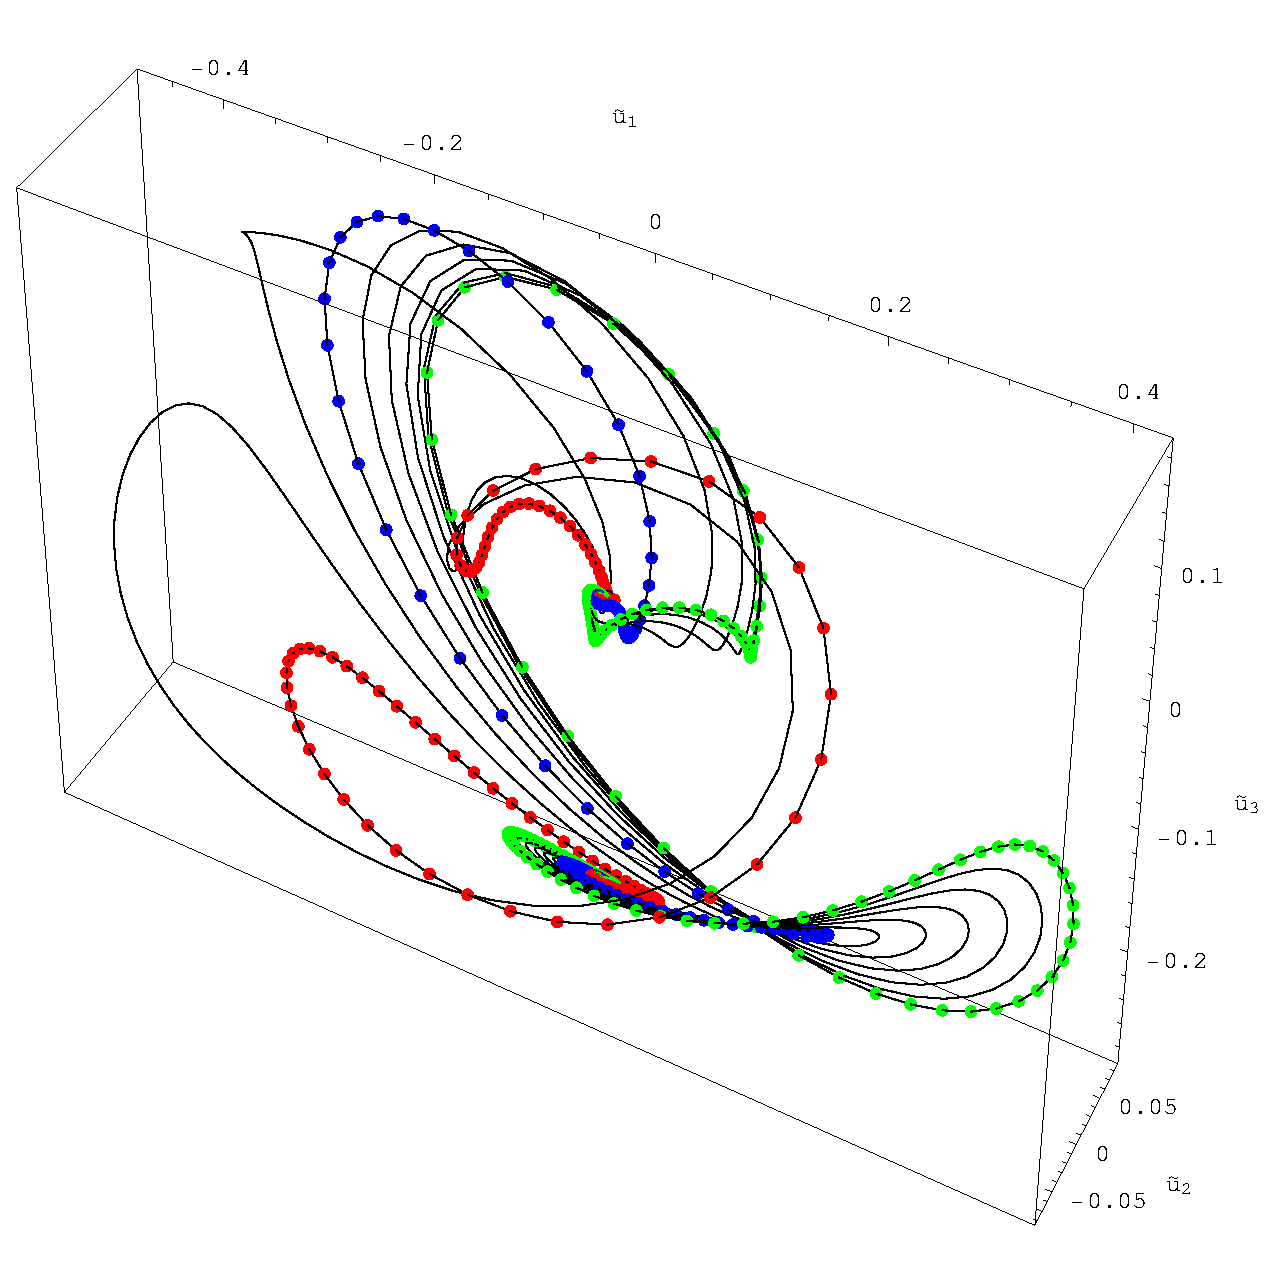
\includegraphics[width=5.0cm]{figs/L22-2w-UnsMan.eps}
\hspace{0.1in}
(b) 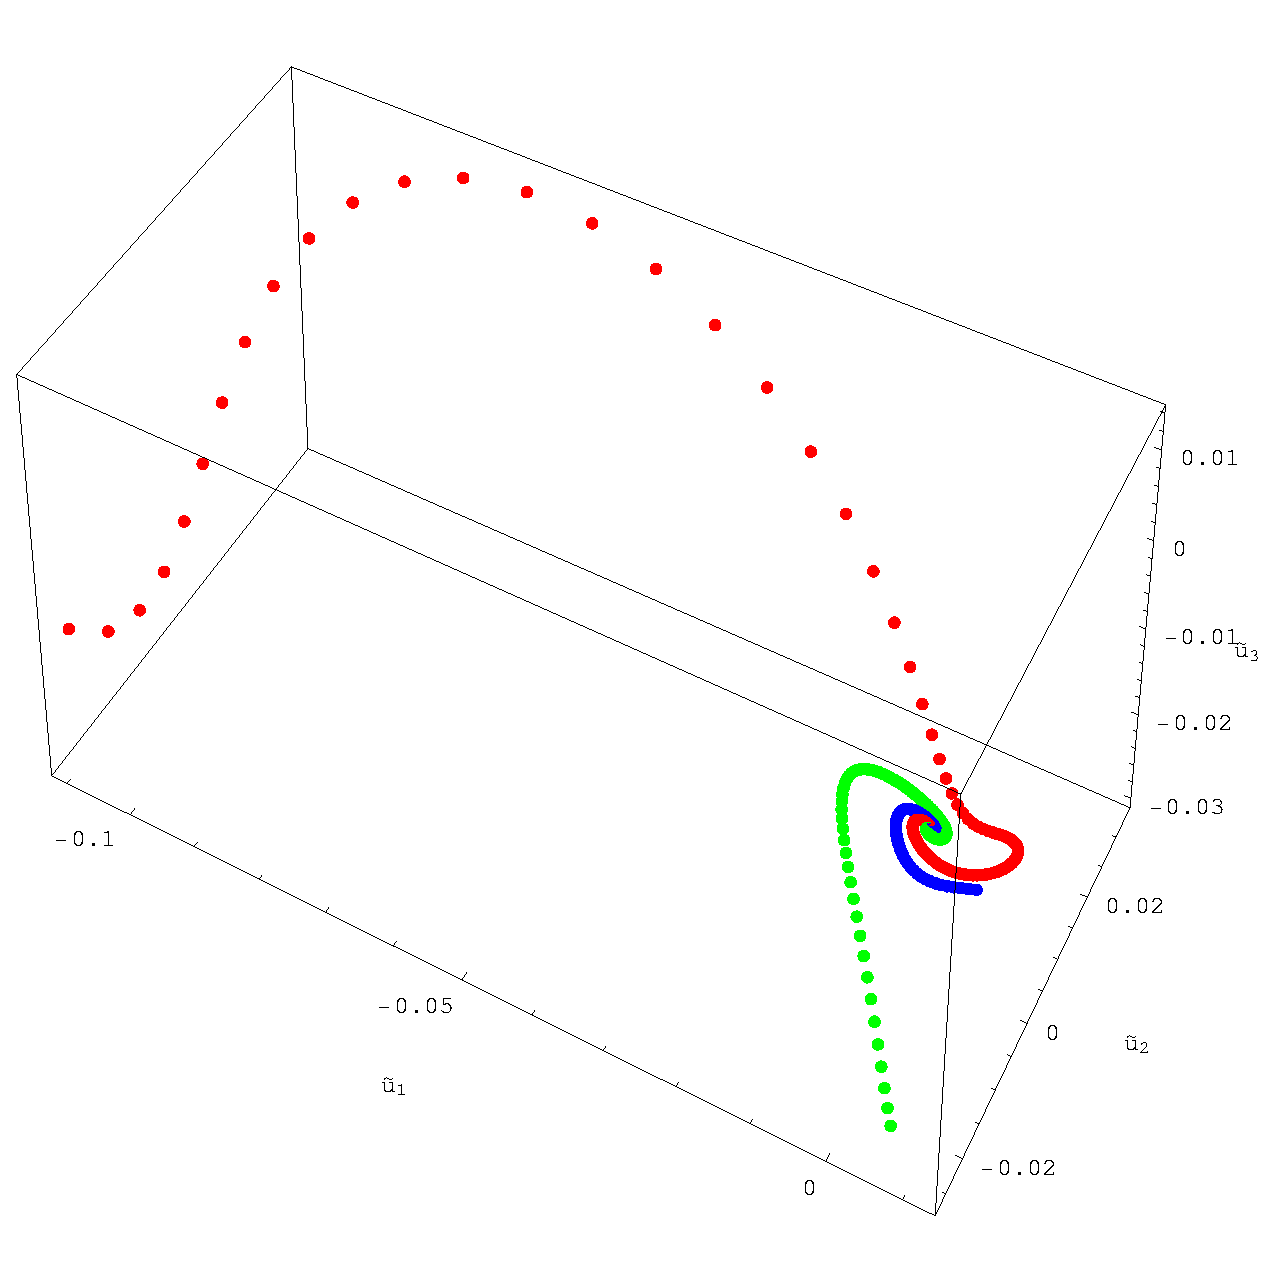
\includegraphics[width=5.0cm]{figs/L22-2w-UnsMan-BlowUp.eps}
% (b) 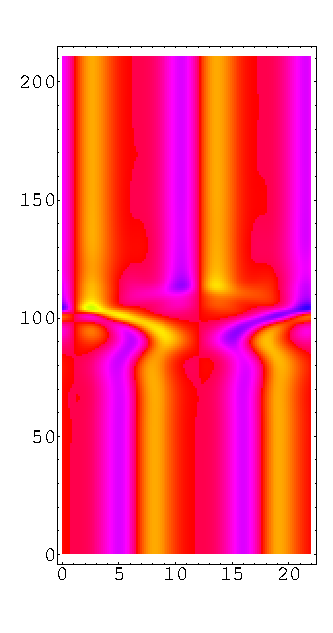
\includegraphics[width=4.0cm]{figs/L22-2w-R.eps}
\\
(c) 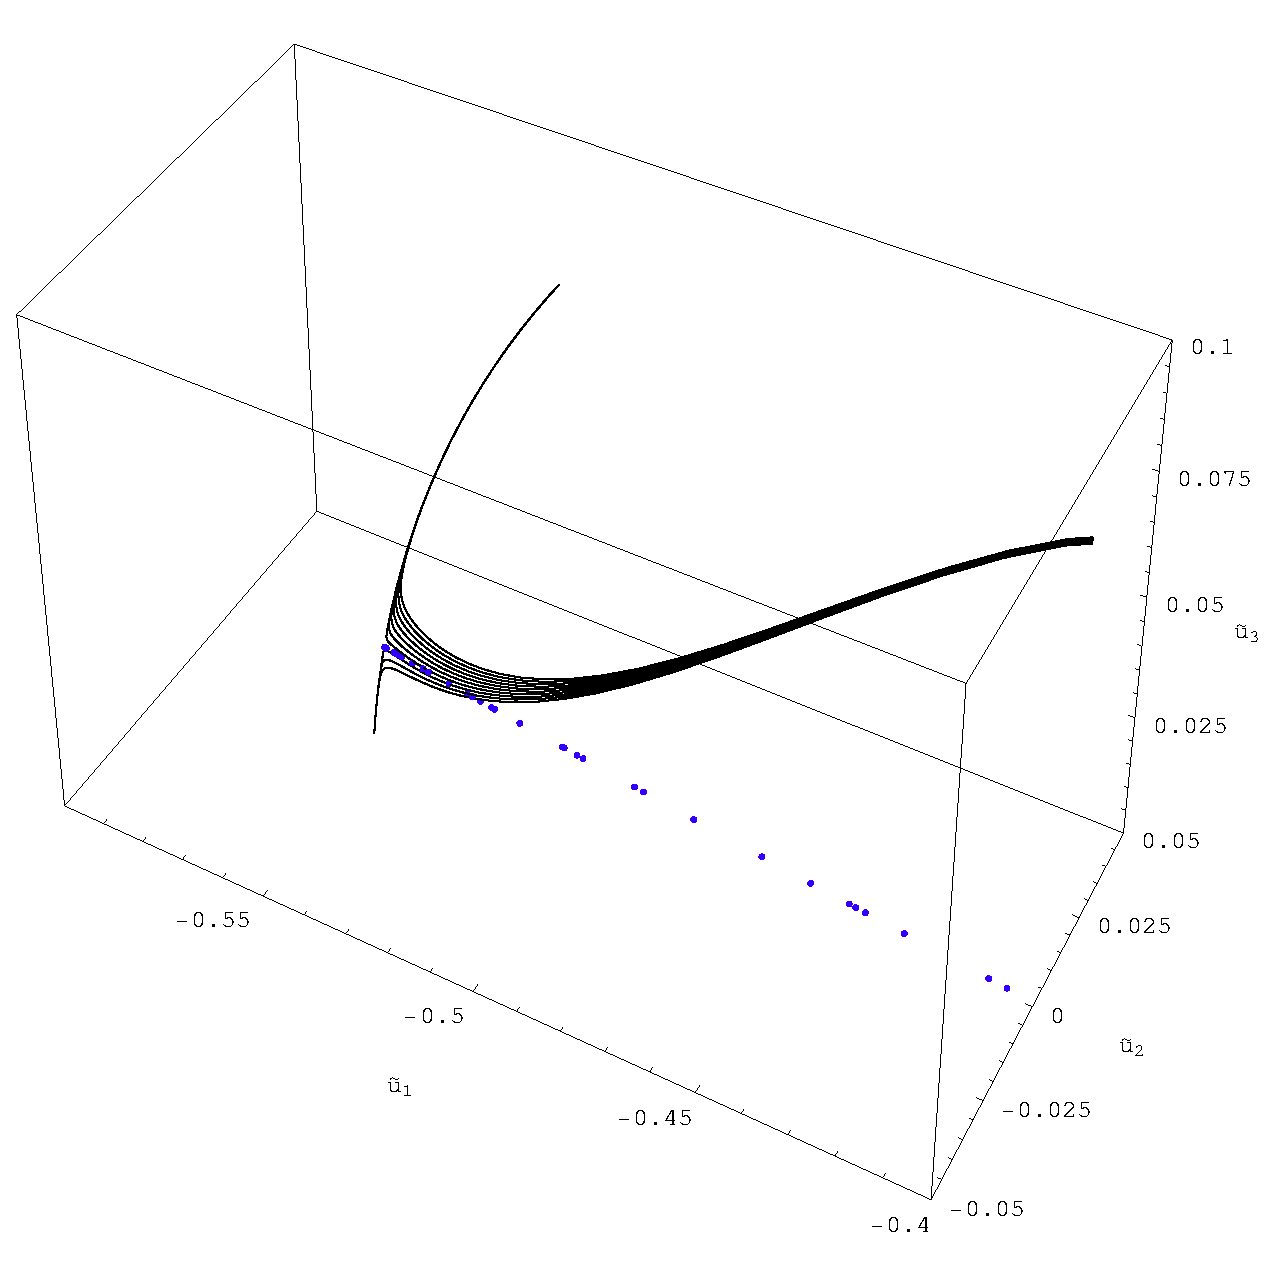
\includegraphics[width=5.0cm]{figs/L22-2w-3w-UnsMan.eps}
% (c) 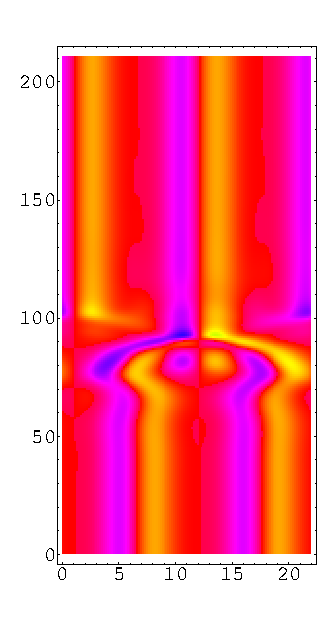
\includegraphics[width=4.0cm]{figs/L22-2w-G.eps}
\hspace{0.1in}
(d)  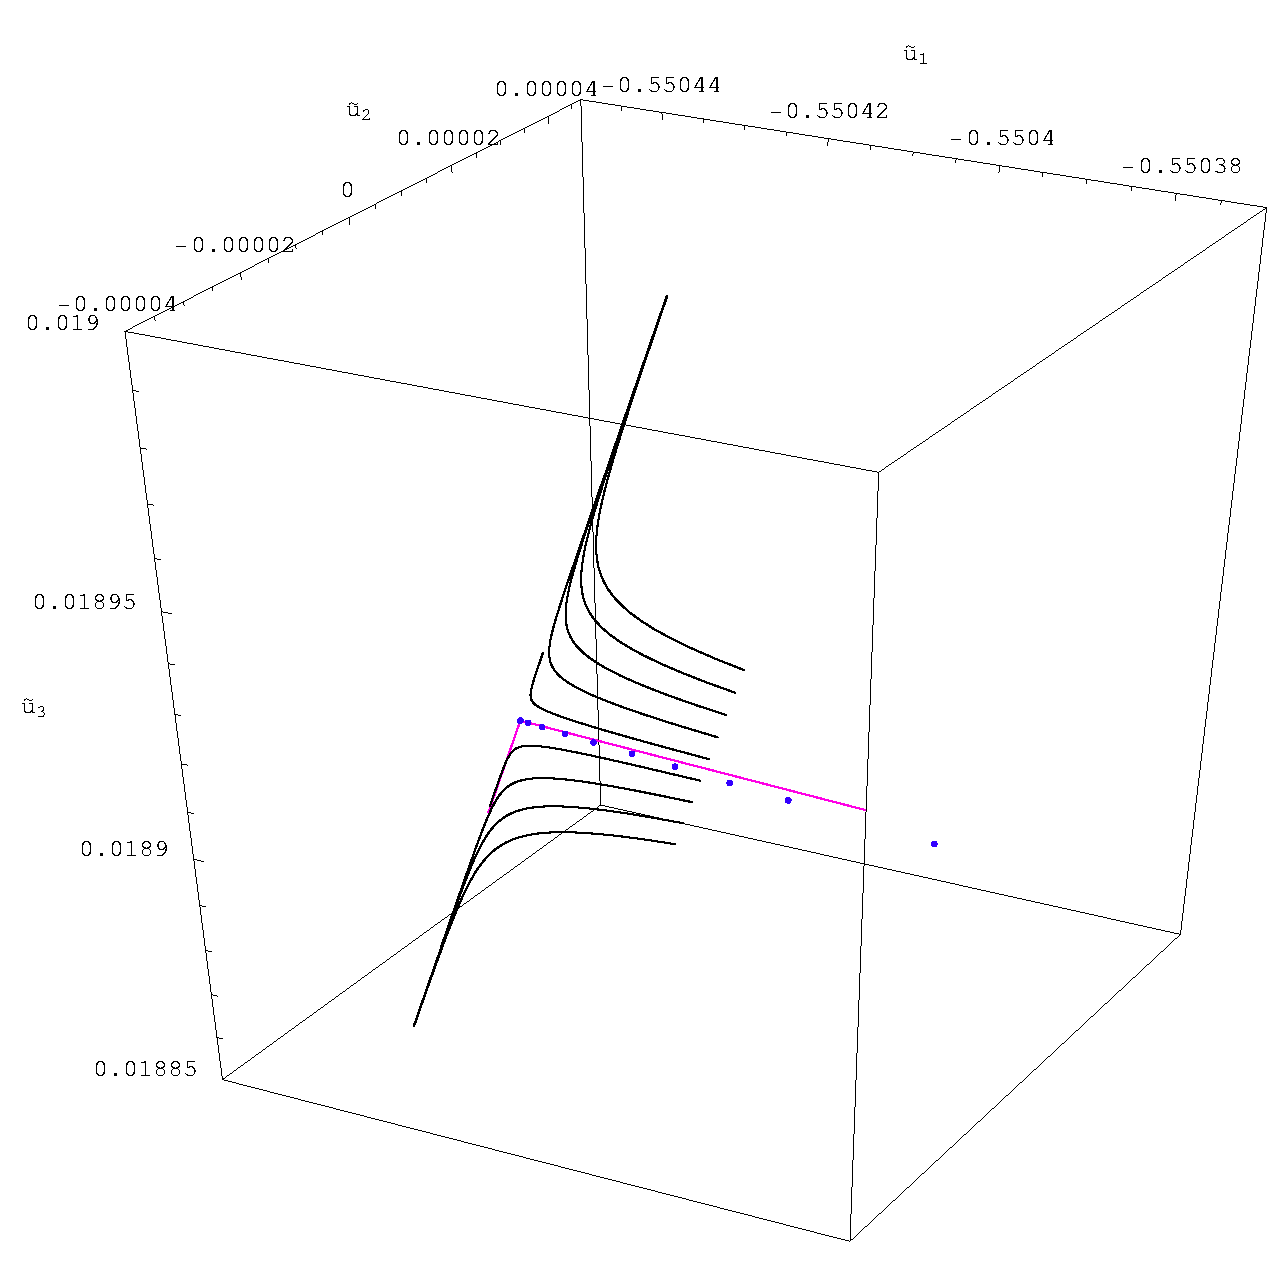
\includegraphics[width=5.0cm]{figs/L22-2w-3w-detail.eps}
% (d) 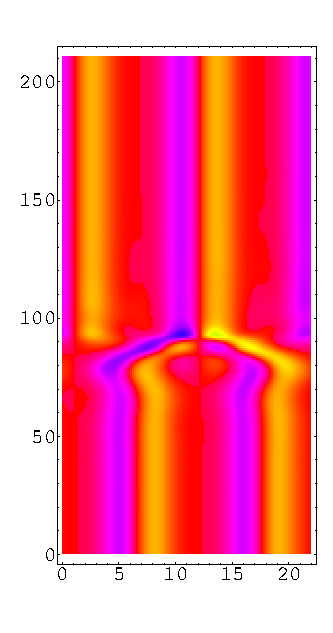
\includegraphics[width=4.0cm]{figs/L22-2w-B.eps}
\caption{
 Trajectories with initial conditions on the unstable subspace of
 the two wavelength equilibria.  
 (a) The coordinates $\tilde{u}_1$ and $\tilde{u}_2$ are along the directions defining the unstable subspace
 and $\tilde{u}_3$  is along the real part of the eigenvector, 
 corresponding to the eigenvalue $-0.271122+ i\, 0.356307$. The purple points represent the continous family
 of two-wavelength equilibria.
% Green curve belongs to \reffig{f:rpo55}(b) % rpo22-55-4-cm.eps
% rather than to  \reffig{f:rpo55}(a), % rpoEq22-55-4.eps?
(b) blowup of ``homoclinic'' descent of the unstable manifold
back into {\nameit}-2 equilibrium, shifted by
$L/4 =5.5$.
(c) blowup of ``heteroclinc'' connection from 
{\nameit}2 \eqv\ to {\nameit}3 \eqv\, with shift 
$L(1/3-1/4) = L/12 = 1.83$ (? check)
to the neighborhood of the point near which the
unstable manifold of the 2-wavelength \eqv\ splits. The blue points
represent the 3-wavelength equilibrium family.
The descent is along the eigenvector of $\Lyap_4= 0.413$ (checked by ES),
and spliting
occurs along one of the 
$\Lyap_1=\Lyap_2=0.0933$
unstable directions of the 3-wavelength equilibrium (checked by ES).
d) same as (c), closer to the 3-wavelength equilibrium. The eigendirections corresponding to $\Lyap_1$
and $\Lyap_4$ are shown in purple. 
}
\label{f:neighborhood2w}
\end{figure}
%%%%%%%%%%%%%%%%%%%%%%%%%%%%%%%%%%%%%%%%%%%%%%%%%%%%%%%%%%%%%%%%%%


\subsection{\Reqva}

Numerical solution of the \reqv\  condition,
transported by travelling wave velocity $c$, 
fixed by the solution for the travelling wave equation:
\[
f_k(u) - i{2\pi\over L} c k u_k = 0
\]

\underline{1-\reqv\  (travelling wave).}
% Ruslan L Davidchack, 	10 Jul 2006 
There is a pair of \reqva\ 
${\nameit}1L$,
${\nameit}1R$
(traveling waves), dual under the
$u(x) \to -u(-x)$ symmetry. They are 
determined numerically by 
adiabatic continuation from a smaller system size
$L~\approx 12$,
where they are stable, to $L=22$
where their velocity is atypically large, $c=7.???$,

Their exponents are:
\\
$\Lyap_i \pm \theta_i =
(
\\
  0.1156222 \pm 0.817289,	\\
  0.033663 \pm 0.418909,	\\
 0.0                    ,	\\
 -0.245729                    ,	\\
 -0.321321 \pm 0.98126,
\cdots
)$

The pair of \reqva\ 
${\nameit}2L$,
${\nameit}2R$
exists for larger system sizes, but does not continue 
adiabatically\rf{saddks} down to $L=22$.

\subsection{\Rpo s}

\ES{
The names of the \rpo\ figure files follow the convention
 {\tt rpoL-T-d.eps}s, with suffixes {\tt cm}
and {\tt u} indicating
 mean velocity frame  and $u$ representation respectively.
   }
%
Out of 30 \rpo s they
find,  only three are truly periodic.  The orbit
with $\period{p} = 95.25$ has a very small
$d = -6.5\,e^{-7}$, but it is not periodic 
(they
checked this by decreasing the integration step size and increasing the
number of modes).

The dynamics in this small system is competition between wavenumbers
2 and 3. The 2-\eqv\  and the 3-\eqv\  essentially lie in
the 2nd and 3rd Fourier component complex plane, with very
small deformations from higher harmonics.
Hence plot all \rpo s in these 2 representations:

$[ \Re a_2, \Im a_2, \Re a_3 ]$
(here 2-\eqv\  is a circle, 3-\eqv\ a vertical line)
 and
$[ \Re a_3, \Im a_3, \Re a_2 ]$
(here 3-\eqv\ is a circle, 2-\eqv\ a vertical line)

This stuff is hard to visualize... for ordinary periodic orbits one
plots the unstable plane of the \eqv, shows where the periodic
orbits sit. Other options:

Somewhat better visualization is in the
{\em mean velocity frame}, {\ie} 
a reference frame that rotates with with velocity 
$v_p=d_p/\period{p}$
In the mean velocity frame a \rpo\ becomes
a \po.
Mean velocity frame visualization helps quite a bit.
Put a black (green, respectively) dot
twice thicknes of the line every time unit; it will enable you to see
where the motion is slow and where it is fast.
% (a trick we used to understand plane Couette trajectories).
Mark the inital point on both
mean velocity \rpo\ and on \eqv\  in mean velocity
 frame with a fat triangle
indicating the direction, so we can see how they both move. Probably at the
opposite ends of the two curves - mean velocity frame is the mean motion.

%   rpo/figs/detail1rpo22-55-4.eps
%   rpo/figs/detail2rpo22-55-4.eps
%   rpo/figs/detail3rpo22-55-4.eps
%   break rpo22-55-4 into 3 parts.
%   The script for the fonts somehow crops these images

Each {\rpo} has its own mean velocity frame - and within it, {\eqv}
move on circles (or worse - because in higher Fourier modes they do mmore
complicted things), and it is important to know where the equlibrium is at
a given instant.

As the shift $d$ is defined mod~$L$, better to
state for each {\rpo} its mean velocity $c_p = d_p/\period{p}$,
where $d_p$ is measured on the line (not on the circle). $c_p$ is
preferrable to angle $2\pi d_p/L$ as it does not vary in $L \to$~large 
limit (just like $\sqrt{2}$ wavelength estimate is independent of
system size.

The \rpo\ {\nameit}55 travels between the 2-\eqv\  and 
2-\eqv\ shifted,
with period and shift
$\period{p}=55.5953\,,\ d=5.24725$
Compared to $L/4 = 5.5$
this is nice, but why not close to periodic after 2nd return? Why 4th return?

The {\nameit}2 {\eqv}
captures qualitatively the mean velocity frame \rpo\ {\nameit}55 shape,
which follows the
equilibrium for most of the time, except for a quick swing where it
sidesteps by $d/4$, just as it does in \reffig{f:rpo55}. 

\Rpo\ {\nameit}55 looks similar to Davidchack's  orbit
of period 
$\period{p}=47.64$ and $d=5.6759$. The period appears to depend on how
many times the orbit manages to spiral around the \eqv.
For {\nameit}55 that appears to be
1.5 times per period, rather than 2. This would led as
to
think there is a family of \rpo s along with a 3rd unit eigenvalue of
$gJ$,
but such does not exist.
So there has to be a selection mechanism corresponding to
reaching or missing the neighborhood of an \eqv\  point starting from
the neighborhood of the other. 

The $u$ space time evolution \reffig{f:rpo55u} % rpo22-55-4-u.eps 
is plotted with the same starting instant,
so one can also track also the spatial profile $u$ in parallel with
the Fourier space projections.

So it is almost impossible to see \reffig{f:rpo55}(b) %rpo22-55-4-cm.eps
in \reffig{f:rpo55}(a) % rpo22-55-4.eps.
I can see 4 periods in \reffig{f:rpo55}(a), %po22-55-4.eps,
but not in \reffig{f:rpo55}(b) %rpo22-55-4-cm.eps
where it comes back only after full period $\period{p}=55.6$.

It still seems that it could be made relative periodic 
(modulo a reflection symmetry?)
in $\period{p}/4=55.6/4=13.9$? That would be OK 
-
by symmetry the figure 8 connecting
2 symmetric equilibria could consist of 4 identical segments: from
equilibrium A to midplane, then reflected version of the same to SA, and
back again.

\Eqv\ are solutions of 3-$d$ set of ODEs  \refeq{eq:3dks}, so
another convenient way to plot \eqva\ and \reqva\ on a periodic
domain $L$ is to plot 
$\partial u(x)$ vs. $u(x)$ as a curve parametrized by
$x\in [0,L]$. In this representation both \eqva\ and \reqva\ curves are
stationary, but the points on \reqva\ move as functions of time.

\Po s and \rpo s can be plotted this way as well
$\partial u(x,t)$ vs. $u(x,t)$. Now they are are represented by time-dependent
``tube".



%%%%%%%%%%%%%%%%%%%%%%%%%%%%%%%%%%%%%%%%%%%%%%%%%%%%%%%%%%%%%%%%
\begin{figure}[t] %[h]
\centering
 	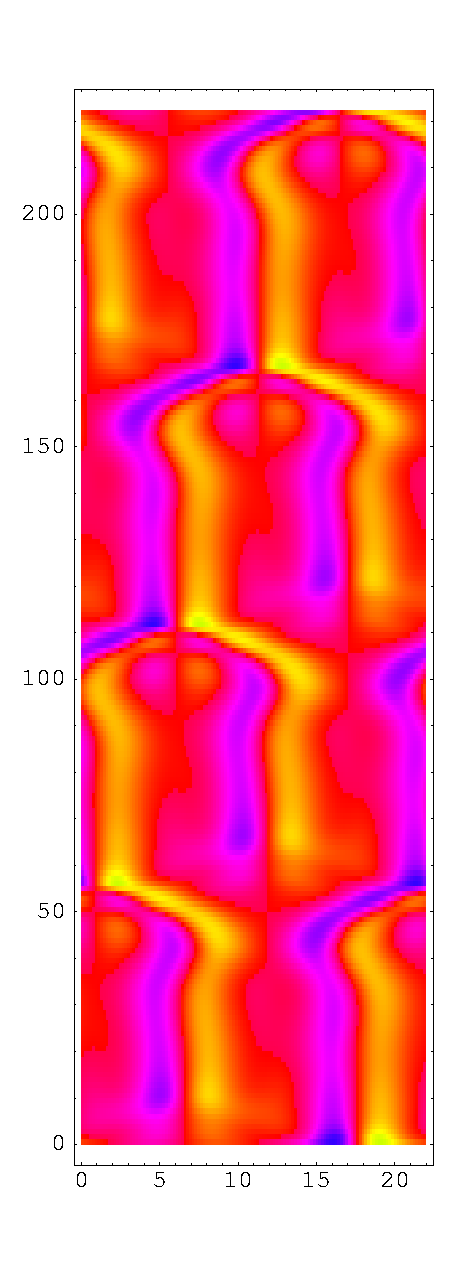
\includegraphics[width=2.5cm]{figs/rpo22-55-4-u.eps}
\hspace{0.1in}
\caption{
 The \rpo\ {\nameit}55 in $u(x,t)$ representation. 
        }
\label{f:rpo55u}
\end{figure}
%%%%%%%%%%%%%%%%%%%%%%%%%%%%%%%%%%%%%%%%%%%%%%%%%%%%%%%%%%%%%%%%%%


%%%%%%%%%%%%%%%%%%%%%%%%%%%%%%%%%%%%%%%%%%%%%%%%%%%%%%%%%%%%%%%%
\begin{figure}[t] %[h]
\centering
(a) 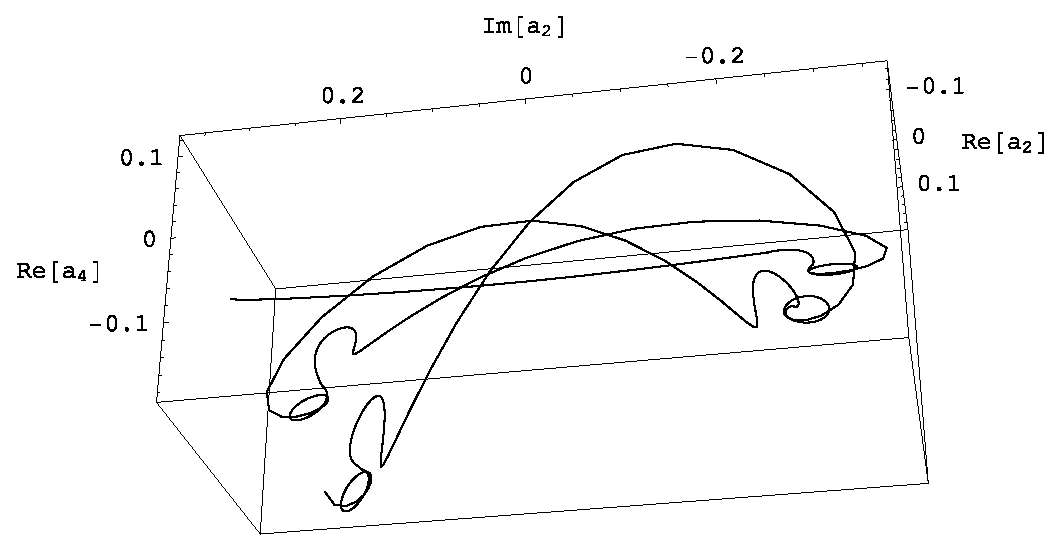
\includegraphics[width=8.0cm]{figs/rpo22-55-4-clean.eps}
% ./removecache.sh rpo22-55-4.eps
% abandoned rpoEq22-55-4.eps with mean velocity equilibrium embeded.
%
\hspace{0.1in}
(b) 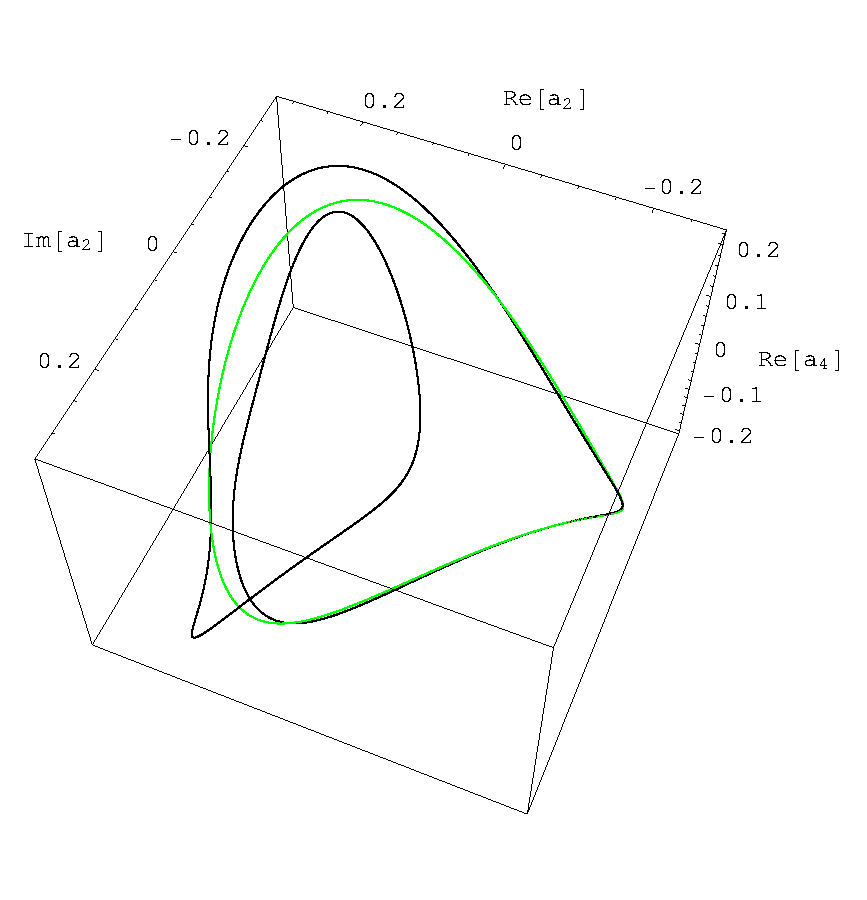
\includegraphics[width=6.0cm]{figs/rpoEq22-55-4-cm.eps}
\\
(c) [create rpoEq22-55-4-cm-?.eps]
\caption{
 The \rpo\ {\nameit}55 in: 
 (a) Phase space, traced for four periods $\period{p}$.
% Green curve belongs to \reffig{f:rpo55}(b) % rpo22-55-4-cm.eps
% rather than to  \reffig{f:rpo55}(a), % rpoEq22-55-4.eps?
 (b) mean velocity frame. 
        The continuos family of 
	equilibria A obtained by the action of $g$ is shown in green,
	the SA family shown in red. The \rpo\ {\nameit}55 stays close
	to either A or SA for close to 1/2 of equilibrum rotation
	period, then quickly jumps to the other equilibrium point.
 (c) mean velocity frame A, SA and {\nameit}55 projected on the 
	$[a_?,a_?]$ plane,
	with the $\sigma x = -x$ symmetry of \KSe\ explicit.
        }
\label{f:rpo55}
\end{figure}
%%%%%%%%%%%%%%%%%%%%%%%%%%%%%%%%%%%%%%%%%%%%%%%%%%%%%%%%%%%%%%%%%%


The two equilibria
capture qualitatively the mean velocity frame \rpo\ {\nameit}55 shape,
which follows the
equilibrium for most of the time, except for a quick swing where it
sidesteps by $d/4$, just as it does in \reffig{f:rpo55}. 

Please also plot it in plane, chose small Fourier coefficients
 which respect the $x \to -x$ symmetry of \KSe.
Then the symmetry of 2 mean velocity
equilibria and self-dual symmetry of \rpo\ {\nameit}55 will be explicit.

Eigenvalues of \rpo\ {\nameit}55 $g\jMps$: are
\\
$(-57.17,  1, 1, -0.500, -0.012, \cdots)$ .
%
%  Eigenvalues of the Jacobian without rotation
%  84.15, -33.86 + 28.94 i, c.c. , 0.48, 0.00019
% no good - missing marginal ones

plots:
  76 rpo60fm23.jpg	\\
 909 rpo60fm23.emf	\\
% Ruslan L Davidchack, 	10 Jul 2006 
the 55 rpo, or whichever seems easiest to explain:
$\period{} = 59.89$,
$c_p = d_p/\period{p}= ?$

$(\ExpaEig_i e^{\pm i\theta_i})=
(
\\
 -27.03397007874626,
\\
   9.34426620337976,
\\
   1
\\
   1
\\
  -0.05018967056231,
\\
   0.00015065158255,
)$

The eigenvectors
indicate that an amplitude mode comes paired with the 
group shift-invariant mode $\ExpaEig_4 =1$. It probably says that
the amplitude $|u_k|$ of the associated can be easily perturbed (think of
a large system: $|u(x)|$ can be easily deformed by long wavelength
perturbations. This \underline{must} be understood. Proposal:

There are two
marginal eigenvalues, one for time translation, one for
rotational invariance. 
The sign of $\ExpaEig_{1}=-57$ says this is a Moebius-kind orbit,
inverse hyperbolic.
Lyapunov $\Lyap=0.07$ says that this neighborhood is much less repelling than
the central equilibrium A, a better candidate for being embedded into the
ergodic attractor.

The \rpo\ initial condition is
so accurate the orbit in \reffig{f:rpo55}(b)
start visibly deviating after retracing the loop 6.5 times.
% the largest unstable multiplier is 
% $-57.17$ per period of the orbit - error would grow to $\approx 60^7
% = 2,800,000,000,000$.

For the \rpo s the accuracy of Jacobian depends
on the time step size, and long runs are needed to refine the results

For a numerical check of the \rpo\ stability eigenvalues,
used two inital
points along an unstable eigenvector $\jEigvec{1}$
at radial distance  $\approx 10^{-4}$ from the \eqv\ {\nameit}2,
and the initial inter-point separation $\Delta(0) \approx 10^{-5}$.
Integrated for time equal to the period $\period{p}=26.3556$ as calculated from
the \jacobianM\ and computed the leading Lyapunov exponent from the ratio of
final to initial distance 
$\Lyap= {1 \over \period{}}\ln( \Delta(\period{})/\Delta(0))$.
Get
$\Delta(\period{})/\Delta(0) =39.01$,
$\Lyap=0.13902$, in agreement with the \eqv\ {\nameit}2 
expanding eigenvalue $\Lyap=0.13904$
\[
\ExpaEig_{radial} =  e^{\Lyap \period{}} =38.99
\,.
\]

% Ruslan L Davidchack, 	10 Jul 2006 
The orbit RLD found has period 60 
rather than 55.  Because it comes so close to the steady states, 
this is probably a numerical precision error.
\\
plots:
 180 rpos1.jpg	\\
1594 rpos1.emf	\\


Rewrite Fourier modes as $u_k(t) = e^{r_k(t) + k(\theta_k(t))}$, study
dynamics and Jacobinas in the $\dot{r_k},\dot{\theta_k})$ representation.
$2$- and $3$-equilibria are nearly cirlces in this representation - higher
modes will not wind wildly if represented by $\theta_k(t)$? Kind of WKB
representation.

period 77 rpo jumps between the two steady states.
\\
plots:	\\
  84 rpo77fm23.jpg	\\
1133 rpo77fm23.emf	\\
 176 rpos2.jpg	\\
1594 rpos2.emf	\\

